\documentclass[12pt,a4paper]{article}

\usepackage[brazilian]{babel}
\usepackage[left=3cm,top=3cm,right=2cm,bottom=2cm]{geometry}
\usepackage{amssymb}
\usepackage{amsmath}
\usepackage{indentfirst}
\usepackage{graphicx}
\usepackage{float}
\usepackage{subcaption}
\usepackage{booktabs}
\usepackage[hidelinks]{hyperref}

\graphicspath{ {../images/} }

\newcommand{\bd}[1]{\textbf{#1}} %bold
\newcommand{\bb}[1]{\bar{\textbf{#1}}} %bar - bold

\title{(Universidade de São Paulo)\\
Pêndulo Simples e Pêndulo Duplo}

\author{Métodos Numéricos em Equações Diferenciais\\
Docente: Fabrício Simeoni de Sousa\\[.2cm]
\begin{tabular}{r@{\ }c@{\ }l}
    Kainã Alves Tureso      &-- &15466391\\
    Vinícius de Sá Ferreira &-- &15491650
\end{tabular}}

\date{\today}

\begin{document}
    \maketitle

    \tableofcontents

    \begin{abstract}
        A modelagem e a simulação numérica de sistemas dinâmicos são fundamentais para a compreensão de fenômenos mecânicos lineares e não lineares. Analisa-se o comportamento do pêndulo simples e do pêndulo duplo sob a ótica de métodos numéricos aplicados a equações diferenciais ordinárias. Para o pêndulo simples, realiza-se o mapeamento das regiões de estabilidade absoluta e a determinação da ordem de convergência dos métodos de Euler explícito, Euler implícito e Runge-Kutta clássico de quarta ordem (RK4), validando os resultados em comparação direta com a solução analítica exata obtida via funções elípticas de Jacobi. Para o pêndulo duplo, formulado a partir do Hamiltoniano do sistema, investiga-se a evolução temporal das trajetórias por meio do método RK4, contrastando o comportamento regular e quase periódico em vizinhanças de equilíbrio estável com a sensibilidade extrema às condições iniciais, característica típica de regimes caóticos determinísticos.
    \end{abstract}

    \section{Pêndulo Simples}
    \subsection{Modelagem e forma padrão}
    O movimento de um pêndulo simples isento de dissipação é governado pela equação diferencial ordinária de segunda ordem
    \begin{equation}
        q''(t) + \sin\bigl(q(t)\bigr)=0,\qquad 
        q(0)=\frac{\pi}{4},\quad q'(0)=0.
    \end{equation}
    A introdução da variável complementar $p(t)=q'(t)$ possibilita a redução para um sistema de primeira ordem na forma padrão
    \begin{equation}
        \bd{u}'(t)=\bd{f}\bigl(\bd{u}(t)\bigr),\qquad
        \bd{u}(t)=\begin{pmatrix} q(t)\\ p(t) \end{pmatrix},\qquad
        \bd{f}(\bd{u})=\begin{pmatrix} p\\ -\sin q \end{pmatrix},
    \end{equation}
    sob a condição inicial $\bd{u}(0)=\bigl(\pi/4,\;0\bigr)^\top$.

    \subsection{Métodos numéricos}
    Definindo $h>0$ como o passo de integração temporal, $t_n=nh$ e $\bd{U}^n\approx\bd{u}(t_n)$ como a aproximação discreta, são considerados três esquemas de integração:

    \begin{description}
        \item[Euler explícito:] $\bd{U}^{n+1}=\bd{U}^n+h\bd{f}(\bd{U}^n)$.
        \item[Runge-Kutta clássico de 4$^{\text{a}}$ ordem (RK4):] 
        \begin{align*}
            \bd{K}_1&=\bd{f}(\bd{U}^n),\\
            \bd{K}_2&=\bd{f}\bigl(\bd{U}^n+\tfrac{h}{2}\bd{K}_1\bigr),\\
            \bd{K}_3&=\bd{f}\bigl(\bd{U}^n+\tfrac{h}{2}\bd{K}_2\bigr),\\
            \bd{K}_4&=\bd{f}\bigl(\bd{U}^n+h\bd{K}_3\bigr),\\
            \bd{U}^{n+1}&=\bd{U}^n+\frac{h}{6}\bigl(\bd{K}_1+2\bd{K}_2+2\bd{K}_3+\bd{K}_4\bigr).
        \end{align*}
        \item[Euler implícito:] $\bd{U}^{n+1}=\bd{U}^n+h\bd{f}(\bd{U}^{n+1})$. A equação não linear resultante é resolvida iterativamente pelo método de Newton a cada passo temporal. Definindo o operador $\bd{F}(\bd{U})=\bd{U}-\bd{U}^n-h\bd{f}(\bd{U})$, a matriz Jacobiana correspondente é expressa por
        \begin{equation}
            \bd{F}'(\bd{U})=\bd{I}-h\bd{J}(\bd{U}),\qquad 
            \bd{J}(\bd{U})=\begin{pmatrix}0&1\\ -\cos q&0\end{pmatrix}.
        \end{equation}
        O passo iterativo é dado por $\bd{U}^{(k+1)}=\bd{U}^{(k)}+\boldsymbol\delta_k$, com o sistema linear associado $\bd{F}'(\bd{U}^{(k)})\boldsymbol\delta_k=-\bd{F}(\bd{U}^{(k)})$, adotando-se como aproximação inicial $\bd{U}^{(0)}=\bd{U}^n$ e critério de parada estabelecido por $\|\boldsymbol\delta_k\|_2<10^{-7}$.
    \end{description}

    \subsection{Estabilidade dos métodos}
    Devido à natureza não linear da equação fundamental, a análise de estabilidade absoluta é realizada por meio de uma linearização local baseada no primeiro termo da série de Taylor da função $\bd{f}$. Esse procedimento viabiliza a determinação dos limites críticos do passo temporal $h$ necessários para assegurar a estabilidade dos integradores.
    
    As regiões de estabilidade absoluta para os referidos métodos, expressas em termos do parâmetro complexo $z = h\lambda$, correspondem aos domínios que satisfazem as seguintes condições:
    \begin{itemize}
        \item Euler explícito: $|1+z| < 1$
        \item RK-4: $\left|1 + z + \dfrac{z^2}{2} + \dfrac{z^3}{6} + \dfrac{z^4}{24}\right| < 1$
        \item Euler implícito: $|1-z| > 1$
    \end{itemize}
    
    Define-se a perturbação local como $\bd{v}(t) := \bb{u} + \bd{u}(t)$, em que o vetor $\bb{u} = (\bar{u}_1, \bar{u}_2)^\top$ assume um estado fixado. Disso decorre que $\bd{v}'(t) = \bd{u}'(t)$. Dado que o sistema em análise é autônomo, tem-se a identidade $\bd{f}(\bd{u}(t), t) = \bd{f}(\bd{u}(t))$, permitindo expressar a dinâmica da perturbação como:
    \begin{align}
        \bd{v}'(t) = \bd{f}(\bb{u} + \bd{v}(t)) \notag
    \end{align}
    A expansão de $\bd{f}$ em série de Taylor em torno do ponto de operação $\bb{u}$ fornece:
    \begin{align}
        \bd{v}'(t) = \bd{f}(\bb{u}) + \bd{f}'(\bb{u})\bd{v}(t) + \mathcal{O}(||\bd{v}||^2) \notag
    \end{align}

    Ao desconsiderar os termos de ordem superior ($\mathcal{O}(||\bd{v}||^2)$), obtém-se um sistema linear não homogêneo. A partir dessa formulação linearizada, determinam-se as condições para a estabilidade absoluta. A matriz jacobiana correspondente assume a forma:
    \begin{align}
        \bd{f}'(\bb{u}) = \begin{bmatrix}
            0 & 1 \\
            -\cos(\bar{u}_1) & 0
        \end{bmatrix} \notag
    \end{align}

    Considerando a condição inicial $q(0) = \frac{\pi}{4}$, pressupõe-se que a imagem da posição angular esteja contida no intervalo $\text{Im}(q) \subset \left[\frac{-\pi}{4}, \frac{\pi}{4}\right]$, fundamentando-se no princípio físico de que o sistema não experimenta ganho de energia mecânica ao longo do tempo. Os valores assumidos pela componente $\bar{u}_1$ coincidem com os estados admissíveis de $q$, intervalo no qual a função cosseno é estritamente positiva. Consequentemente, os autovalores da matriz $\bd{f}'(\bb{u})$ são determinados por $\lambda_1 = i \sqrt{\cos(\bar{u}_1)}$ e $\lambda_2 = -i \sqrt{\cos(\bar{u}_1)}$. 

    Verifica-se que $\lambda_1$ e $\lambda_2$ constituem números imaginários puros, cujas amplitudes são delimitadas pelas faixas $\Im(\lambda_1) \in \left[ \frac{1}{\sqrt[4]{2}}, 1\right]$ e $\Im(\lambda_2) \in \left[-1, -\frac{1}{\sqrt[4]{2}}\right]$. Posto que o passo de integração cumpre a condição $h\in \mathbb{R}_{>0}$, os valores assumidos por $z$ localizam-se inteiramente sobre o eixo imaginário. Com base nesses fundamentos, estabelecem-se os critérios de estabilidade aplicáveis a cada método.

    Para o método de Euler explícito, sendo os produtos $z_i = h\lambda_i$ ($i=1,2$) puramente imaginários, a relação $|1 + z_i| = \sqrt{1^2 + \Im(z_i)^2} > 1$ mantém-se válida para qualquer $z_i \ne 0$. Por conseguinte, constata-se que o esquema explícito manifesta instabilidade irrestrita para o cenário considerado, logo nenhum $h > 0$ satisfaz a condição de estabilidade.

    Para o método de Euler implícito, sob o mesmo princípio algébrico, demonstra-se que a condição $|1-z_i| > 1$ é rigorosamente satisfeita para todo $i=1,2$. Desse modo, o esquema caracteriza-se como incondicionalmente estável, logo qualquer $h > 0$ satisfaz a condição de estabilidade.

    Para o método Runge-Kutta de quarta ordem (RK4), a avaliação restringe-se à interseção da região de estabilidade com o eixo imaginário. Definindo $z=ia$ com $a \in \mathbb{R}$ e substituindo-o na expressão que delimita a fronteira de estabilidade, obtém-se:
    \begin{align}
        \left|1 + ia - \dfrac{a^2}{2} - \dfrac{ia^3}{6} + \dfrac{a^4}{24}\right| < 1 \notag
    \end{align}
    A eliminação do operador radical na norma complexa resulta na inequação equivalente:
    \begin{align}
        \left(1-\dfrac{a^2}{2} + \dfrac{a^4}{24}\right)^2 + \left(a - \dfrac{a^3}{6}\right)^2 < 1 \notag
    \end{align}
    A resolução analítica dessa inequação estabelece o intervalo de confinamento $|a| \in (0,\; 2\sqrt{2})$. Sendo $|a_j| = |h \cdot \Im(\lambda_j)| \le h$, conclui-se diretamente que $|z_j| \le h$. Portanto, para assegurar a estabilidade absoluta do integrador RK4 em uma vizinhança de $\bb{u}_1 \in \left[\dfrac{-\pi}{4}, \dfrac{\pi}{4}\right]$, o passo de integração temporal deve cumprir a restrição $h \in (0,\; 2\sqrt{2})$. 

    \subsection{Estratégias de implementação}
    A geração da solução de referência fundamenta-se em formulações analíticas expressas por meio de funções elípticas de Jacobi, implementadas via rotinas predefinidas (\texttt{RefSolution.py}). Para o modelo do pêndulo simples, fixa-se o tempo final de simulação em $T=15$. A quantificação do erro e a verificação da ordem de convergência realizam-se a partir de cinco malhas de amostragem uniforme, caracterizadas pelos passos discretos $h = 0.1,\; 0.05,\; 0.01,\; 0.005,\; 0.001$. O erro global é avaliado com base na norma do supremo da diferença entre a solução numérica e a solução analítica de referência mapeada no último nó temporal da simulação.

    \subsection{Resultados e discussão}
    \subsubsection{Posição angular no tempo}
    A evolução temporal da variável de estado $q(t)$, obtida por meio dos três esquemas numéricos empregando o passo $h=0.05$, encontra-se disposta nas Figuras~\ref{fig:pos_tempo_sob} e~\ref{fig:pos_tempo}. Constata-se um alinhamento rigoroso entre a trajetória de referência e a gerada pelo integrador RK4. Em contrapartida, o método de Euler explícito exibe um crescimento artificial e acentuado da amplitude de oscilação, enquanto o método de Euler implícito manifesta um decaimento rápido (amortecimento numérico), ratificando os resultados deduzidos na análise de estabilidade linear.

    \begin{figure}[H]
        \centering
        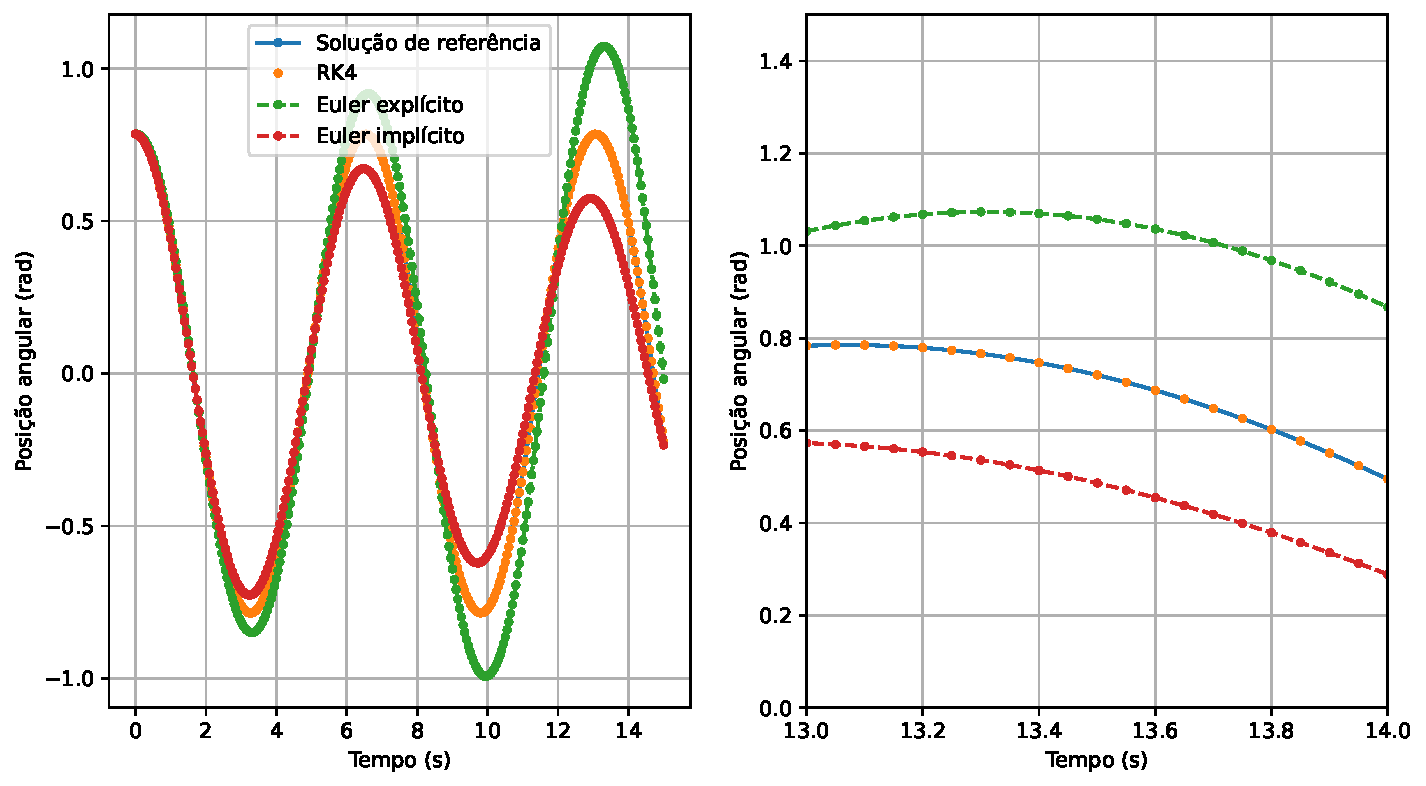
\includegraphics[width=0.8\linewidth]{Comparacao_p_simples.pdf}
        \caption{Comparação sobreposta de posição angular $q(t)$ para $h=0.05$ e $T=15$.}\label{fig:pos_tempo_sob}
    \end{figure}

    \begin{figure}[H]
        \centering
        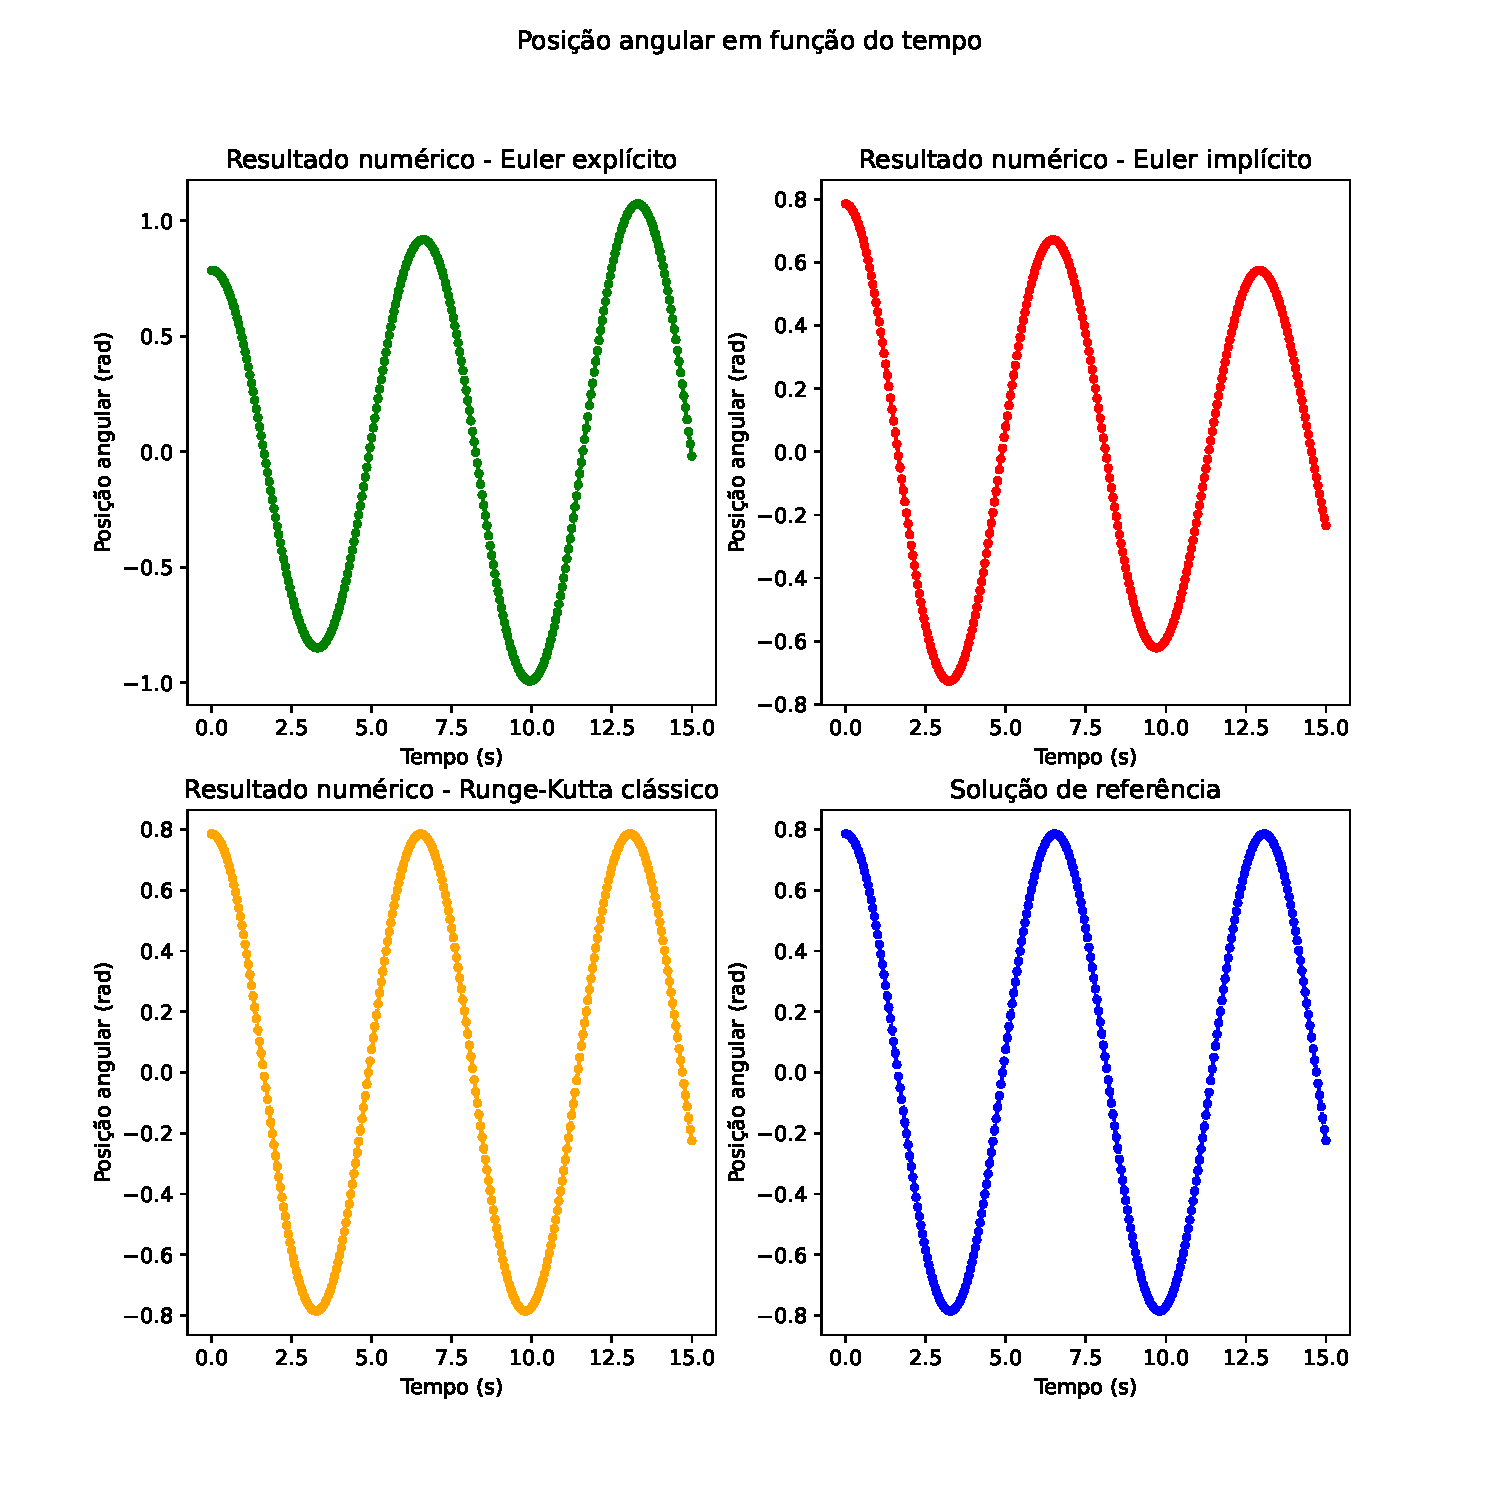
\includegraphics[width=0.8\linewidth]{p_posxtempo.pdf}
        \caption{Posição angular $q(t)$ para $h=0.05$ e $T=15$.}\label{fig:pos_tempo}
    \end{figure}

    \subsubsection{Ordem de convergência}
    A avaliação do comportamento do erro global frente ao refinamento da malha temporal evidencia as propriedades assintóticas de cada integrador. As curvas de erro relativas ao método de Euler explícito (Figura~\ref{fig:err_exp}) e ao método de Euler implícito (Figura~\ref{fig:err_imp}) revelam perfis lineares com inclinação unitária em escala log-log, confirmando a primeira ordem de convergência teórica. Paralelamente, a Figura~\ref{fig:err_rk4} demonstra um declive coincidente com o valor 4, validando a precisão de quarta ordem característica do algoritmo RK4. Tais perfis comprovam a convergência assintótica dos erros para zero conforme o passo $h\to0$.

    \begin{figure}[H]
        \centering
        \begin{subfigure}{0.32\textwidth}
            \centering
            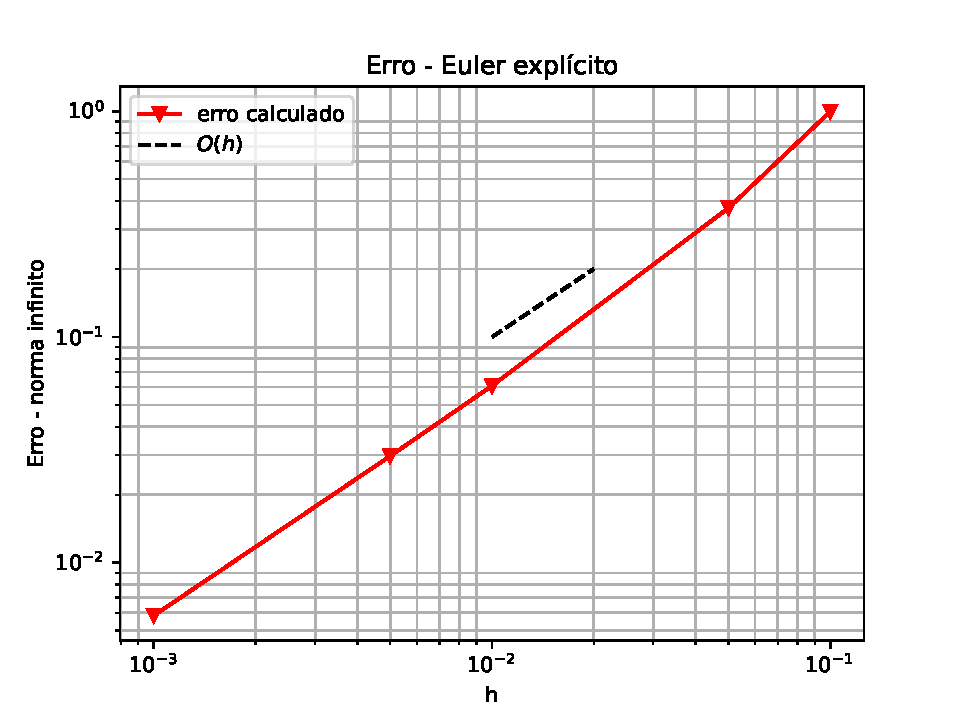
\includegraphics[width=\linewidth]{erro_explicito.pdf}
            \caption{Euler explícito}\label{fig:err_exp}
        \end{subfigure}
        \begin{subfigure}{0.32\textwidth}
            \centering
            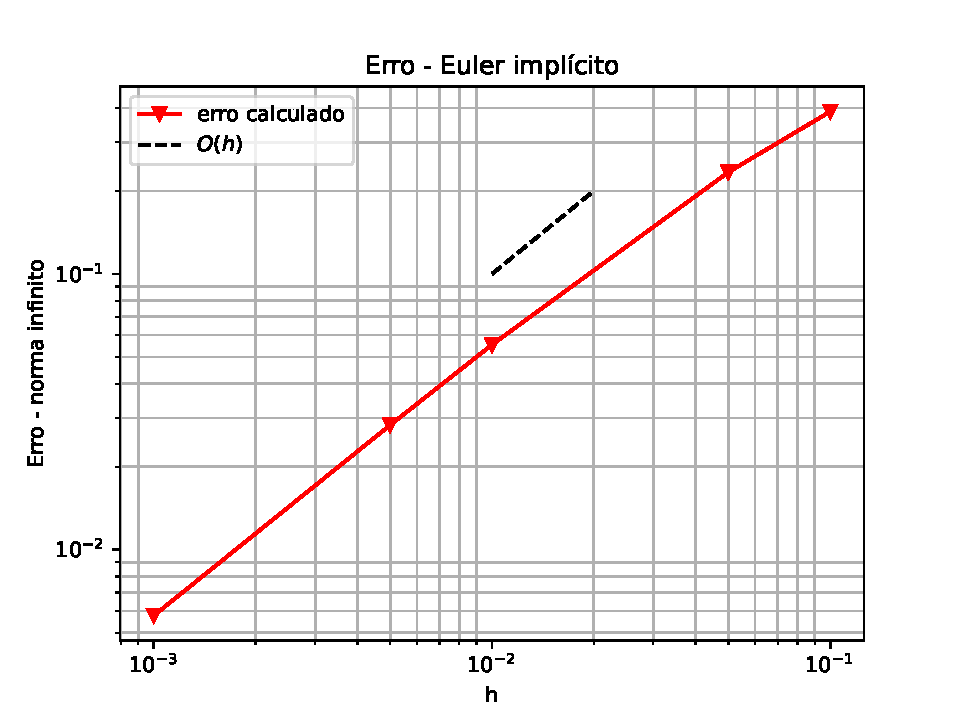
\includegraphics[width=\linewidth]{erro_implicito.pdf}
            \caption{Euler implícito}\label{fig:err_imp}
        \end{subfigure}
        \begin{subfigure}{0.32\textwidth}
            \centering
            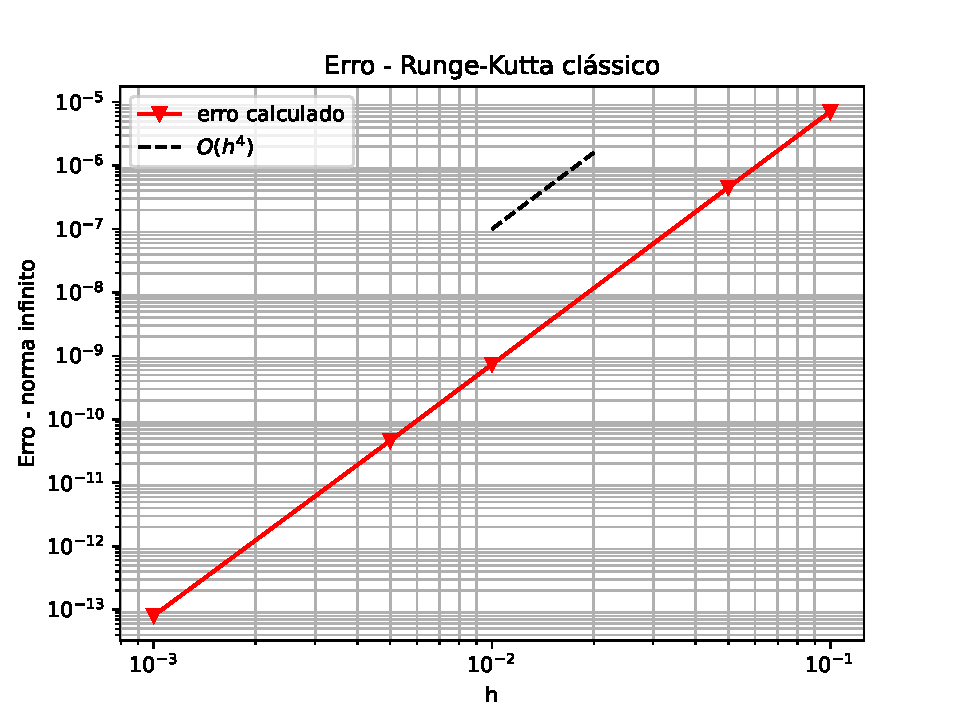
\includegraphics[width=\linewidth]{erro_RK4.pdf}
            \caption{RK4}\label{fig:err_rk4}
        \end{subfigure}
        \caption{Erro global em função do passo $h$ (escala log-log).}
    \end{figure}

    \subsubsection{Retrato de fase}
    O mapeamento das trajetórias no espaço de estados $(q,p)$ correspondente à solução de referência é ilustrado na Figura~\ref{fig:retrato}. Devido ao caráter estritamente periódico do movimento e à conservação da energia mecânica total, o comportamento ideal traduz-se em uma órbita perfeitamente fechada, padrão este preservado de forma consistente pelo método RK4. Por outro lado, os diagramas associados aos métodos de Euler revelam perfis espiralados, expondo o ganho ou a dissipação espúria de energia mecânica decorrente das propriedades de estabilidade intrínsecas a cada formulação discreta.

    \begin{figure}[H]
        \centering
        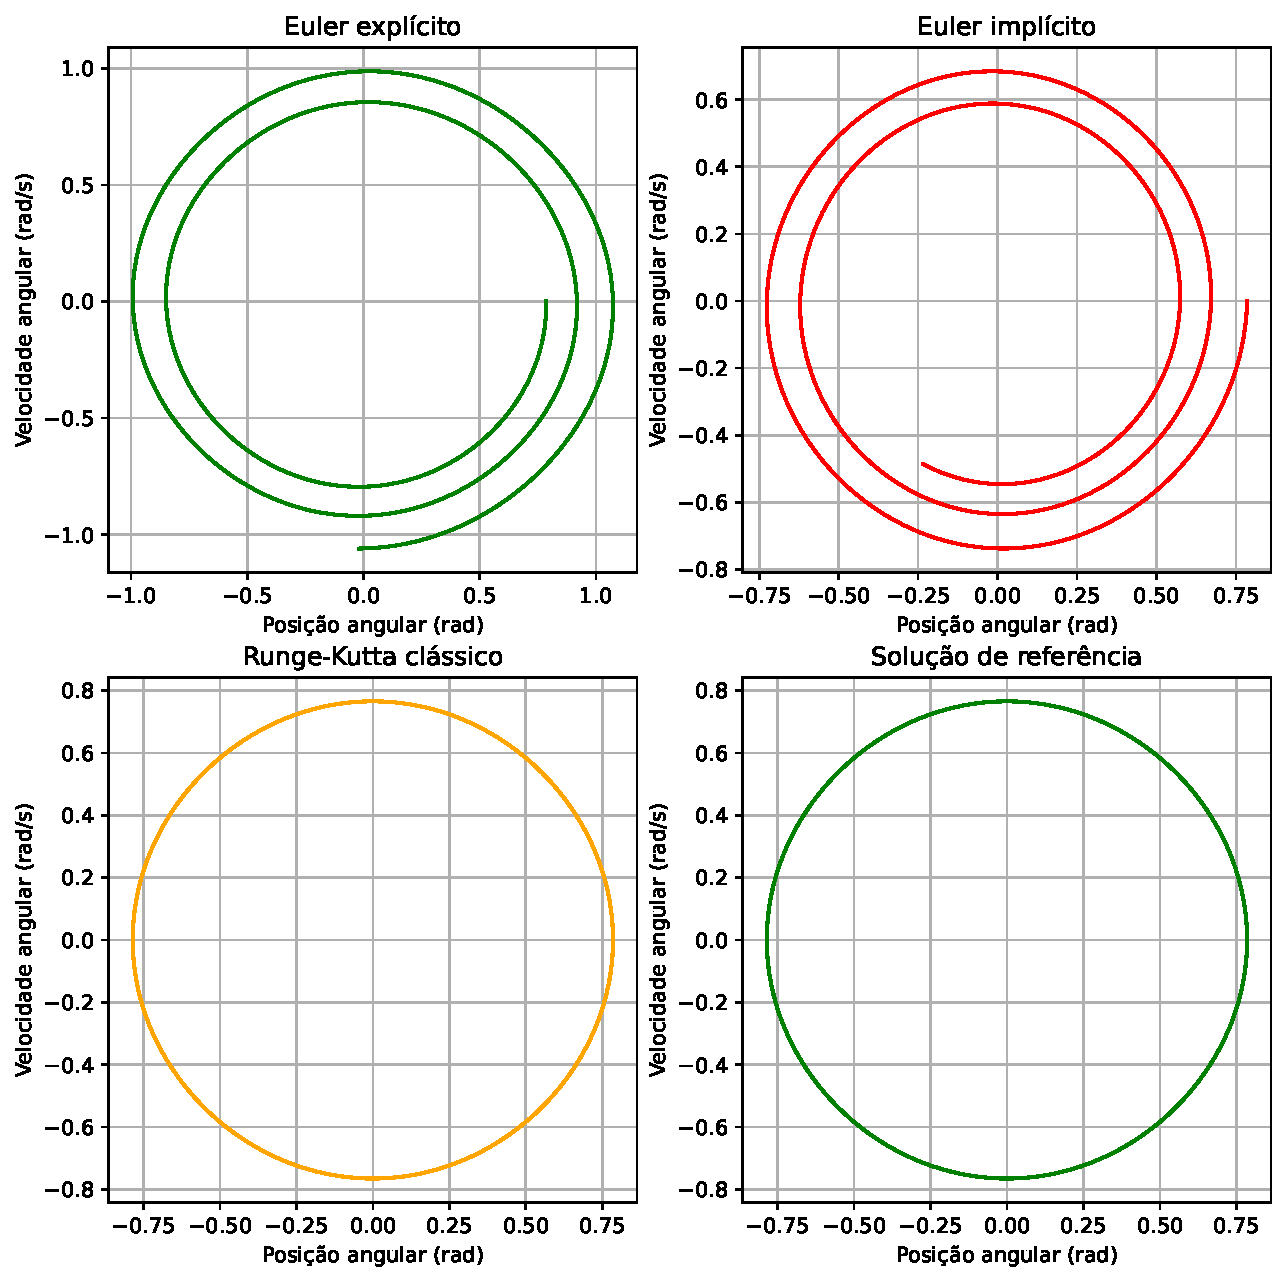
\includegraphics[width=0.62\linewidth]{retrato_fase.pdf}
        \caption{Retrato de fase (posição angular $(q)$ $\times$ velocidade angular $(p)$).}\label{fig:retrato}
    \end{figure}

    \section{Pêndulo Duplo}
    \subsection{Modelagem e sistema de EDOs}
    O sistema mecânico do pêndulo duplo acoplado, considerando massas, comprimentos e aceleração gravitacional unitários, é integralmente descrito pelas coordenadas generalizadas $q_1, q_2$ e seus respectivos momentos conjugados $p_1, p_2$. As equações diferenciais governantes do movimento, deduzidas a partir do formalismo Hamiltoniano, são estruturadas como:
    \begin{align}
        \dot q_1 &= \frac{p_1-p_2\cos(q_1-q_2)}{2-\cos^2(q_1-q_2)}, \\
        \dot q_2 &= \frac{2p_2-p_1\cos(q_1-q_2)}{2-\cos^2(q_1-q_2)}, \\
        \dot p_1 &= -A_1+A_2-2\sin q_1, \\
        \dot p_2 &= A_1-A_2-\sin q_2,
    \end{align}
    onde os termos de acoplamento não linear $A_1$ e $A_2$ são definidos por:
    \begin{align*}
        A_1 &= \frac{p_1p_2\sin(q_1-q_2)}{1+\sin^2(q_1-q_2)}, \\
        A_2 &= \frac{\bigl(p_1^2+2p_2^2-2p_1p_2\cos(q_1-q_2)\bigr)\sin(q_1-q_2)\cos(q_1-q_2)}{\bigl[1+\sin^2(q_1-q_2)\bigr]^2}.
    \end{align*}
    A evolução temporal do sistema é computada por meio do algoritmo RK4, adotando-se um passo de integração fixo $h=0.01$ e tempo final $T=50$. As condições iniciais específicas são parametrizadas de acordo com os ensaios descritos a seguir.

    \subsection{Trajetória do segundo pêndulo}
    A determinação da trajetória espacial descrita pela extremidade livre do segundo pêndulo no plano cartesiano, apresentada na Figura~\ref{fig:traj_q2}, é obtida por meio das relações de transformação cinemática:
    \begin{equation}
        x_1=\sin q_1,\quad y_1=-\cos q_1,\qquad
        x_2=x_1+\sin q_2,\quad y_2=y_1-\cos q_2.
    \end{equation}
    Sob as condições iniciais preestabelecidas $q_1(0)=q_2(0)=3\pi/4$ e $p_1(0)=p_2(0)=0$, observa-se uma dinâmica marcadamente aperiódica, resultando em uma trajetória que preenche densamente uma região compacta do plano.

    \begin{figure}[H]
        \centering
        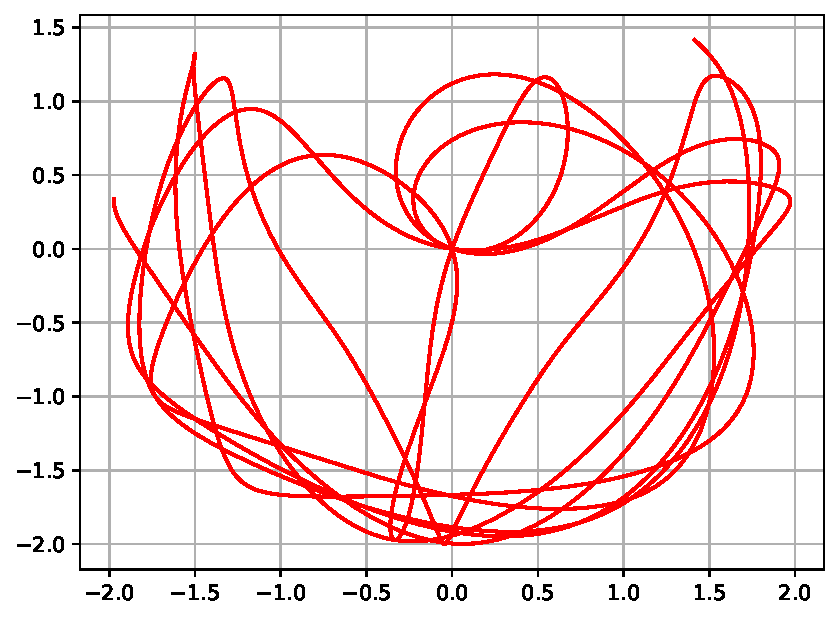
\includegraphics[width=0.6\linewidth]{pendulo_duplo.pdf}
        \caption{Trajetória de $(x_2(t),y_2(t))$ para $q_1(0)=q_2(0)=3\pi/4$, $T=50$.}\label{fig:traj_q2}
    \end{figure}

    \subsection{Experimentos}
    \subsubsection{Condições iniciais próximas ao equilíbrio}
    O primeiro cenário investiga o comportamento dinâmico em uma vizinhança restrita do ponto de equilíbrio estável, adotando $q_1(0)=q_2(0)=0.2$ (regime de pequenas oscilações) e momentos iniciais nulos. Nessas condições, as variáveis de estado permanecem confinadas à proximidade da configuração vertical inferior. A trajetória resultante no plano cartesiano, ilustrada na Figura~\ref{fig:exp1}, caracteriza-se por um padrão geométrico regular, confinado e dotado de propriedades quase periódicas.

    \begin{figure}[H]
        \centering
        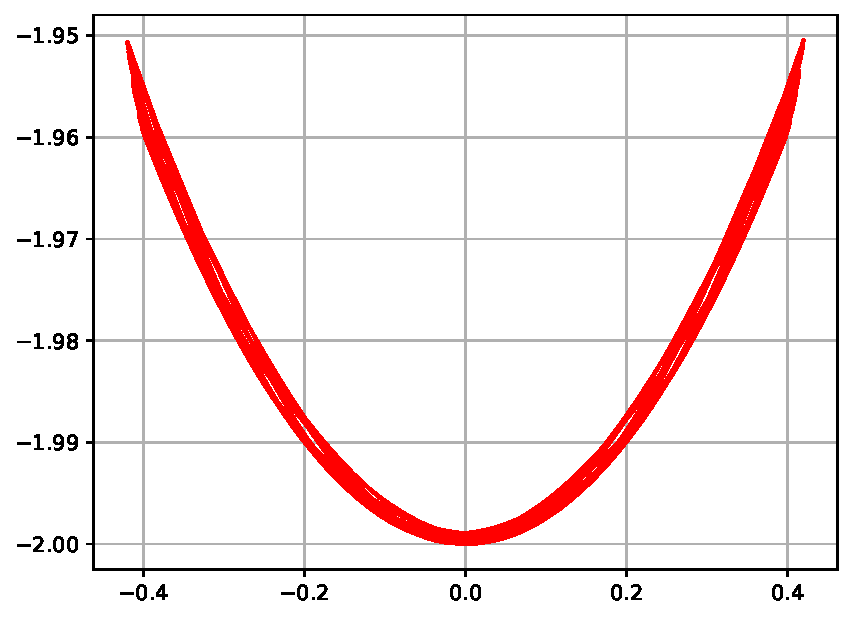
\includegraphics[width=0.6\linewidth]{pendulo_duploeq.pdf}
        \caption{Trajetória de $(x_2,y_2)$ para $q_1(0)=q_2(0)=0.2$.}\label{fig:exp1}
    \end{figure}

    \subsubsection{Comportamento caótico e sensibilidade às condições iniciais}
    No segundo cenário, estabelece-se a configuração angular $q_1(0)=q_2(0)=\pi/2$ como estado de referência. Subsequentemente, introduz-se uma perturbação infinitesimal da ordem de $10^{-2}$ exclusivamente na segunda coordenada angular, definindo-se a condição modificada $q_2(0)=\pi/2+0.01$. As respostas dinâmicas e as trajetórias espaciais geradas para ambos os casos encontram-se confrontadas nas Figuras~\ref{fig:tra_1} e~\ref{fig:tra_2}.

    \begin{figure}[H]
        \centering
        \begin{subfigure}{0.48\textwidth}
            \centering
            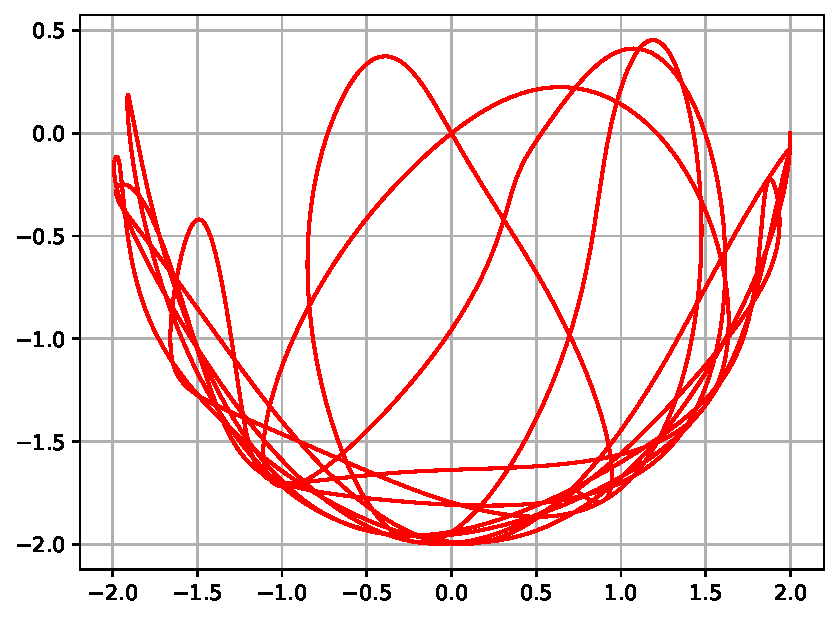
\includegraphics[width=\linewidth]{pendulo_duplo1.pdf}
            \caption{$q_1(0)=q_2(0)=\pi/2$}\label{fig:tra_1}
        \end{subfigure}
        \begin{subfigure}{0.48\textwidth}
            \centering
            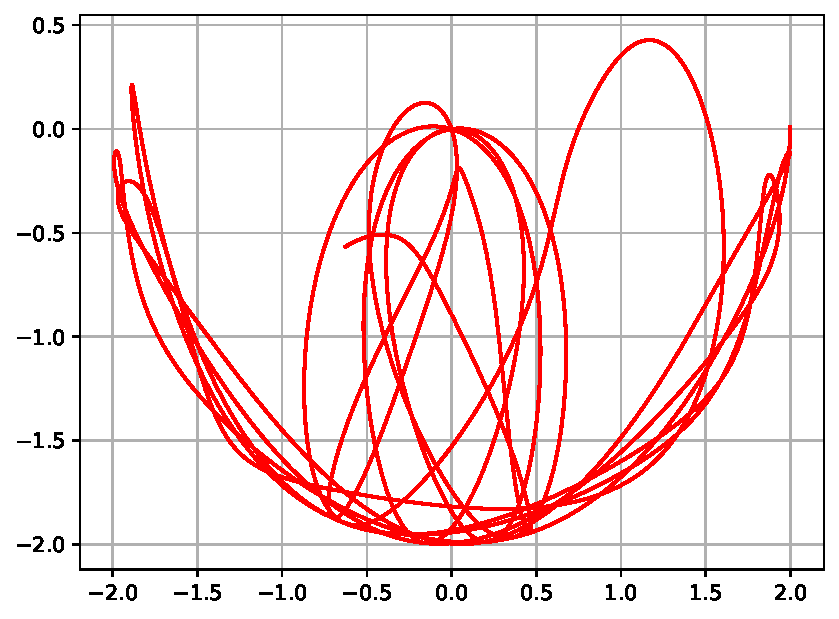
\includegraphics[width=\linewidth]{pendulo_duplo2.pdf}
            \caption{$q_1(0)=\pi/2,\; q_2(0)=\pi/2+0.01$}\label{fig:tra_2}
        \end{subfigure}
        \caption{Comparação das trajetórias $(x_2,y_2)$ com e sem perturbação.}\label{fig:exp2}
    \end{figure}

    A despeito da proximidade extrema entre os estados iniciais, verifica-se uma divergência exponencial e qualitativa das trajetórias após decorrido um curto intervalo temporal, evidenciando de forma inequívoca a sensibilidade extrema às condições iniciais que caracteriza o caos determinístico. A propagação e amplificação rápidas do desvio inicial culminam na formação de topologias de movimento inteiramente distintas. Esse comportamento diferencia-se substancialmente da resposta previsível observada em sistemas lineares ou integráveis, consolidando-se como uma propriedade definidora de sistemas caóticos.
\end{document}